\documentclass[aspectratio=169,usenames,dvipsnames]{beamer}
\usepackage{preamble}
\title{Coding for Humanities, week 4}

% notes
% - add list comprehensions? They are in the notebook

\begin{document}

\begin{frame}
 \titlepage
\end{frame}

\begin{frame}{Last week}
    \large
    Dictionaries

    \vspace{1em}
    Functions

    \vspace{1em}
    Text (pre)processing
\end{frame}

\begin{frame}{Plan for today}
 \tableofcontents
\end{frame}

\section{Exam preparation}
\frame{\tableofcontents[currentsection]}

\subsection{Recap week 1--3}
\begin{frame}[fragile]{Week 1: Values}
    \begin{description}
        \item[Numbers] \lstinline{-1, 2, 3.5}, etc.
        \item[Special] \lstinline{True, False, None}
        \item[Strings] \lstinline{'a', 'hello', "I'm"}
\begin{lstlisting}
"""Multi
line
strings"""
\end{lstlisting}
    \end{description}
\end{frame}

\begin{frame}[fragile]{Week 1: Variables \& arithmetic}
    \begin{description}[Assignment]
        \item[Assignment] \lstinline{name = expression}
        \item[Increment] \lstinline{number += 1}
        \item[Expressions] 1 + 2 * number + int('4')
    \end{description}
    \pause
    \begin{itemize}
        \item Can use \structure{variable} instead of constant
        \item Can use \structure{function} call instead of constant
        \item Expressions are evaluated \structure{step by step}:
    \end{itemize}
\begin{lstlisting}
old = 3
new = 1 + 2 * old + int('4')
# new = 1 + 2 * 3 + int('4')
# new = 1 + 6 + int('4')
# new = 1 + 6 + 4
# new = 7 + 4
# new = 11
\end{lstlisting}
\end{frame}

\begin{frame}[fragile]{Week 2: Sequences}
    \begin{description}[Indexing/slicing]
        \item[Indexing/slicing] \lstinline{seq[0], seq[2:4]}
        \item[Concatenation] \lstinline{seq1 + seq2}
        \item[Length] \lstinline{len(seq)}
        \item[Types] \lstinline{list, str, tuple}
    \end{description}
\end{frame}
\begin{frame}[fragile]{Week 2: Lists}
    \begin{description}[Lists in lists]
        \item[Creation] \lstinline{mylist = [['a', 0], ['b', 1]]}
        \item[Lists in lists]
            \lstinline{mylist[0] == ['a', 0]} \\
            \lstinline{mylist[0][1] == 0}
        \item[Append] \lstinline{mylist.append(['c', 2])}
    \end{description}
\end{frame}
\begin{frame}[fragile]{Week 2: If-statements}
    \begin{description}[Conditions]
        \item[Conditions] \lstinline{a == b, letter == 'a', number < 2, item in seq}
        \item[If]
            \lstinline{if condition: ...}

            \lstinline{elif condition: ...}

            \lstinline{else: ...}
    \end{description}
\end{frame}
\begin{frame}[fragile]{Week 2: Loops}
    \begin{description}[Iterables]
        \item[For-loop] \lstinline{for item in iterable:}\\
            \hspace{1em}\lstinline{# do something with item}
        \pause
        \item[Iterables] \lstinline|list, str, tuple, dict, range()|
        \pause
    \item[For-loop idiom]
\begin{lstlisting}
result = 0  # or []
for item in iterable:
    if item ...:
        # do something with item
        # add to result
\end{lstlisting}
\end{description}
\end{frame}

\begin{frame}[fragile]{Week 3: Dictionaries}
    \begin{description}[creation]
        \item[creation] \lstinline|example = {'a': 0, 'b': 1}|
        \item[lookup] \lstinline{example['a']}
        \item[update] \lstinline{example['a'] = 2} (also for new keys)
    \end{description}
\end{frame}

\begin{frame}[fragile]{Week 3: Functions}
    \begin{description}[Return value]
        \item[Defining] \lstinline{def name(param1, ...): ...}
        \item[Calling] \lstinline{name(arg1, ...)}
        \item[Return value] \lstinline{return ...}
    \end{description}
    \pause
\begin{columns}[T]
\column{0.5\linewidth}
\begin{lstlisting}
# function with effect
def greeting(name):
    print('Hello', name)

greeting('John')
# cannot store greeting with:
x = greeting('John')
\end{lstlisting}
\column{0.5\linewidth}\pause
\begin{lstlisting}
# function with a result
def mean(numbers):
    if not numbers:
        return None
    return sum(numbers) / len(numbers)

print(mean([7, 8]))
x = (mean([6, 8]) + mean([7, 8])) / 2
\end{lstlisting}
\end{columns}
\end{frame}
\begin{frame}[fragile]{Week 3: Strings}
    \begin{description}[Formatting]
        \item[Lowercasing] \lstinline{lowered = sent.lower()}
        \item[Splitting] \lstinline{tokens = sent.split()}
        \item[Joining] \lstinline{', '.join(seq)}
        \item[Formatting] \lstinline|f'My name is {last}, {first} {last}'|
        \item[Escaping] \lstinline|'newline=\n tab=\t quote=\' slash=\\'|
    \end{description}
\end{frame}

\begin{frame}{Learning to program is learning a language}
\begin{columns}[T]
\column{0.5\linewidth}
Similarities:
\begin{itemize}
	\item Need to memorize \structure{vocabulary}.
	\item Follow \structure{grammar} rules
	\item Practice reading \\
			and especially \structure{writing}.
	\item Recognize and use \structure{idioms}.
	\item Don't be afraid to make mistakes, \\
		you only improve by trying.
\end{itemize}
    \column{0.5\linewidth}
\pause Differences:
\pause
\begin{itemize}
	\item No ambiguity, subtext, etc.
	\item Only commands, \\
        no description etc.
	\item The computer will not guess \\
        what you are trying to say.
	\item The computer gives \\
        immediate feedback.
\end{itemize}
\end{columns}
\end{frame}

\begin{frame}{Learning to program is learning a language}
Demonstrated by research:

\vspace{1em}
Prat et al 2020.
Relating Natural Language Aptitude to Individual Differences
in Learning Programming Languages.
\url{https://www.nature.com/articles/s41598-020-60661-8}
%\url{https://doi.org/10.1038/s41598-020-60661-8}

\vspace{1em}
    \structure{Bottom line}: language aptitude more important than numeracy
\end{frame}

% list comprehensions!

\subsection{Solutions to exercises}
\begin{frame}{Make 3rd sg form}
The third person singular verb form in English is distinguished by the suffix
-s, which is added to the stem of the infinitive form: run $\rightarrow$ runs.
A simple set of rules can be given as follows:
\begin{enumerate}
    \item If the verb ends in y, remove it and add ies
    \item If the verb ends in o, ch, s, sh, x or z, add es
    \item By default just add s
\end{enumerate}

\vspace{1em}
Hint: Check out the string method \href{https://docs.python.org/3/library/stdtypes.html\#str.endswith}{\lstinline{.endswith()}}.
\end{frame}

\begin{frame}[fragile]{Make 3rd sg form}
\begin{lstlisting}
def make_3sg_form(verb):
    if verb.endswith('y'):
        return verb[:-1] + 'ies'
    elif verb.endswith(('o', 's', 'x', 'z', 'ch', 'sh')):
        return verb + 'es'
    else:
        return verb + 's'
\end{lstlisting}
\end{frame}


\begin{frame}[fragile]{extract\_dialogue}
\scriptsize
\begin{verbatim}
ACT I. Scene I.
Verona. A public place.

Enter Sampson and Gregory (with swords and bucklers) of the house
of Capulet.


  Samp. Gregory, on my word, we'll not carry coals.

  Greg. No, for then we should be colliers.

  Samp. I mean, an we be in choler, we'll draw.
[...]

  Greg. 'Tis well thou art not fish; if thou hadst, thou hadst
    been poor-John. Draw thy tool! Here comes two of the house of
    Montagues.

           Enter two other Servingmen [Abram and Balthasar].


  Samp. My naked weapon is out. Quarrel! I will back thee.
[...]
\end{verbatim}
\end{frame}

\begin{frame}[fragile]{extract\_dialogue}
    Approach:
    \begin{enumerate}
        \item Split paragraphs (given)
        \item Loop over paragraphs (for-loop)
        \item Identify paragraphs with dialogue
        \item Split name and line
        \item Store in dictionary
    \end{enumerate}
\end{frame}

\begin{frame}[fragile]{Identify paragraphs with dialogue?}
\begin{verbatim}
Enter Sampson and Gregory (with swords and bucklers) of the house
of Capulet.


  Samp. Gregory, on my word, we'll not carry coals.
\end{verbatim}

    \vspace{1em}
    What is the difference between the first and last line?

    \pause
    Dialogue starts with an abbreviated character name (`Samp.')
    
    \vspace{1em}
    So, do \lstinline{.split()} and check if first word \lstinline{.endswith('.')}
\end{frame}

\begin{frame}[fragile]{Split name and line?}
\begin{verbatim}
  Samp. Gregory, on my word, we'll not carry coals.
\end{verbatim}

    \vspace{1em}
    Want to split only \structure{once} on first dot.

    \vspace{1em}
    Check documentation at \url{https://docs.python.org/3/library/stdtypes.html\#str.split}

    \vspace{1em}
    \centering
    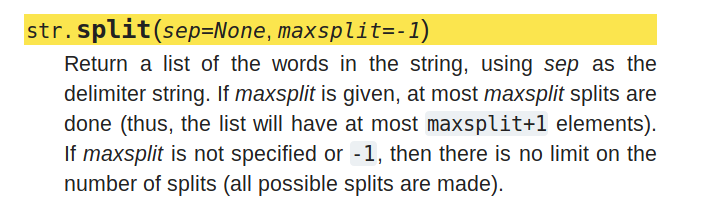
\includegraphics[width=0.9\linewidth]{fig/splitdocs}
\end{frame}

\begin{frame}[fragile]{Clean up extra whitespace?}
    See \url{https://docs.python.org/3/library/stdtypes.html\#str.strip}

    \vspace{1em}
    \centering
    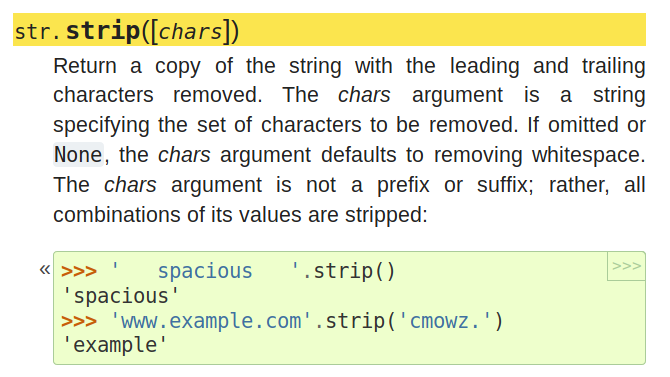
\includegraphics[width=0.9\linewidth]{fig/stripdocs}
\end{frame}

\begin{frame}[fragile]{Store in dictionary?}
    Want to store for each character multiple lines of dialogue.

    \vspace{1em}
    So use a dictionary, keys: character names, values: list of dialogue lines
\begin{lstlisting}
paragraphs = ...
result = {}
# for para in paragraphs:
    # name = ...  # a character name
    # line = ...  # a line of dialogue
    if name not in result:
        result[name] = []
    result[name].append(line)
\end{lstlisting}
\end{frame}

\begin{frame}[fragile]{Putting it all together}
\begin{lstlisting}
def extract_dialogue(text):
    paragraphs = text.split('\n\n')
    result = {}
    for para in paragraphs:
        # paragraphs with dialogue start with
        # a character name and period: 'Samp. ...'
        first_token = para.split()[0]
        if first_token.endswith('.'):
            name, line = para.split('.', 1)
            # remove leading/trailing spaces
            name = name.strip()
            if name not in result:
                result[name] = []
            result[name].append(line)
    return result
\end{lstlisting}
\end{frame}

\begin{frame}{Problem solving strategies}
    \begin{description}
        \item[Bottom up] first work out details, work towards larger program
            \begin{itemize}
                \item Break up problem into smallest practical parts
                \item Solve separately
                \item \structure{Merge} parts until problem is solved
            \end{itemize}
        \item[Top down] start from big picture, \structure{split} into sub-problems \\
            and work towards details
            \begin{itemize}
                \item more structured
                \item requires planning
            \end{itemize}
    \end{description}

    \vspace{1em}
    Either way: if stuck, solve an easier problem first
\end{frame}

\begin{frame}{Types of learning}
    \begin{description}[Implicit learning]
        \item[Explicit learning]
            read slides, textbook, watch lectures.
        \item[Implicit learning]
            \begin{itemize}
                \item learning by doing, try lots of things
                \item learning from examples (osmosis)
            \end{itemize}
    \end{description}

    \vspace{1em}
    Implicit learning is crucial for programming!
\end{frame}

\subsection{Q\&A}
\begin{frame}{Poll}
    \begin{enumerate}
        \item Q1 How much of the week 3 notebook and exercises did you finish?
            \begin{enumerate}
                \item less than 50\%
                \item 50--70\%
                \item 70--80\%
                \item 90--100\%
            \end{enumerate}
        \item Q2 write questions in chat
    \end{enumerate}
\end{frame}



\section{Working with files}
\frame{\tableofcontents[currentsection]}

\begin{frame}{Motivation}
    To do anything non-trivial,

    programs need to work with \structure{arbitrary data}

    \pause
    Therefore, need to learn how to:

	\begin{itemize}
		\item \structure{read} external data(sets) from disk as input,
		\item and \structure{write} results as output
	\end{itemize}

\end{frame}


\begin{frame}{Files and directories}
    \begin{itemize}
        \item Data is stored in \structure{files} as a sequence of bytes
        \item Files are part of \structure{directories} (folders)
        \item Directories may contain files and other directories.\\
            Ergo:
            \begin{itemize}
                \item The file system is a tree structure.
                \item The location of a file is a path through this tree.
            \end{itemize}
    \end{itemize}
\end{frame}

\begin{frame}{Why directories}
    % Motivate organization
    \begin{itemize}
        \item Directories are useful to organize your files
        \item Use short, sensible names
        \item Don't put everything in one big pile. \\
            For example: separate code, data, results
    \end{itemize}
    \pause 
    Learn to use your system's file manager (Finder, Explorer, etc.)
    \begin{itemize}
        \item Make directories
        \item Move/rename files
        \item etc.
    \end{itemize}
    
\end{frame}

\begin{frame}[fragile]{Messy and organized files}
\begin{columns}
\column{0.5\linewidth}
\begin{verbatim}
Untitled 1.pdf
Untitled 1(1).pdf
Untitled 1(2).pdf
Untitled 1(2)(2)_draft.pdf
Untitled 1(2)_draftFINAL.pdf
Untitled 1(2)_FINAL_comments.pdf
Untitled 1(2)_FINAL_REALLY_FINAL.pdf
Untitled 1(2)_FINAL_make_it_stop.pdf
Untitled 1(2)_lAST-mInUtE-ChAnGES.pdf
\end{verbatim}
\pause
\column{0.5\linewidth}
\begin{verbatim}
code/ ...
data/ ...
research/ ...
teaching/ ...
└── codingforhumanities/
    ├── lectures/
    │   ├── slides1.pdf
    │   ├── slides2.pdf
    │   └── fig/ ...
    ├── notebooks/
    │   ├── ...
    │   └── data/ ...
    └── syllabus/
        └── syllabus.pdf
\end{verbatim}
\end{columns}
\end{frame}

\begin{frame}{Paths}
    \begin{itemize}
        \item A path describes the location of a file
		\begin{itemize}
        \item In the simplest case, just the filename is enough to
            refer to a file in the same directory as your program/notebook:

            \texttt{example.txt}

        \item If a file is somewhere else, need to include directories:

            \texttt{data/example.txt}\\
            \texttt{data/novels/19thcentury/austen/emma.txt}
		\item Use .. to refer to the parent directory
		\end{itemize}
    \end{itemize}
    \structure{NB}: Windows uses \textbackslash instead of \texttt{/}. \\
        However, this causes problems, use \texttt{/} in Python!
\end{frame}


\section{Importing modules}
\frame{\tableofcontents[currentsection]}

\begin{frame}
    Until now:
        \begin{itemize}
            \item Language basics
            \item Simple problems
        \end{itemize}
    \pause
    From here on:
        \begin{itemize}
            \item Using existing code
            \item Concrete applications
        \end{itemize}
\end{frame}

\begin{frame}[fragile]{Importing modules}
To go beyond builtin functionality, use import:
\begin{lstlisting}
# import whole module:
import <module>
# or import a specific part:
from <module> import <function>
\end{lstlisting}

\pause
\begin{lstlisting}
In: import math
In: math.pi
Out: 3.141592653589793
In: from math import sqrt
In: sqrt(16)
4.0
\end{lstlisting}

Matter of preference/convention which you use:
\begin{itemize}
    \item \lstinline{math.pi}: clear that pi comes from math module
    \item \lstinline{sqrt}: less typing \dots
\end{itemize}
\end{frame}

\subsection{The Python standard library}
\begin{frame}[fragile]{The Python standard library}
	"Batteries included"

	\vspace{1em}
	Many useful functions

	\vspace{1em}
    See \url{https://docs.python.org/3/library/index.html}
\end{frame}

\begin{frame}[fragile]{Finding files}
    \begin{itemize}
        \item \structure{globbing}: matching a set of files with a search pattern.
        \item The most common operators are:
            \begin{itemize}
                \item \texttt{*} meaning ``match zero or more characters''
                \item \texttt{?} meaning ``match exactly one character''
            \end{itemize}
        %\item The \texttt{glob} module offers pattern matching of files.
        %\item The glob library contains a function also called \texttt{glob}
		%	to match file patterns
        %\item e.g., \texttt{glob.glob('*.txt')} matches all files in the
        %    current directory whose names end with .txt.
    \end{itemize}
\pause
Example:
\begin{lstlisting}
In: from glob import glob
In: glob('Chapter*')
Out: ['Chapter 2 - Basic text processing.ipynb',
    'Chapter 1 - Getting started.ipynb',
    'Chapter 3 - Text analysis.ipynb',]
In: glob('data/*.txt')
Out: ['austen-emma.txt', 'world-domination.txt', 'evil-plans.txt']
\end{lstlisting}
\end{frame}

% \begin{frame}[fragile]{Counter}
% \begin{itemize}
% \item A Counter is a specialized dictionary for counting
% \item values are (integer) counts; missing values are 0
% \item Mathematical term: \structure{bag}, \structure{multiset}
% \end{itemize}
% 
% \begin{lstlisting}
% In: from collections import Counter
% In: cnt = Counter(['the', 'cat', 'is', 'on', 'the', 'mat'])
% In: cnt
% Out: Counter({'the': 2, 'is': 1, 'mat': 1, 'on': 1, 'cat': 1})
% \end{lstlisting}
% \end{frame}
% 
% \begin{frame}[fragile]{Counter: initialization}
% Several ways to initialize a Counter:\\
% 
% \begin{lstlisting}
% In: cnt = Counter()
% In: cnt
% Out: Counter()
% In: cnt = Counter(['red', 'blue', 'red', 'blue', 'red'])
% In: cnt
% Out: Counter({'red': 3, 'blue': 2})
% In: cnt = Counter({'red': 3, 'blue': 2})
% In: cnt
% Out: Counter({'red': 3, 'blue': 2})
% \end{lstlisting}
% \end{frame}
% 
% \begin{frame}[fragile]{Word frequency counting}
% \begin{lstlisting}
% words = [...]       # Some list of words
% counts = {}
% \end{lstlisting}\pause
% \begin{lstlisting}
% for word in words:
%     if word not in counts:
%         counts[word] = 0
%     counts[word] += 1
% ...
% \end{lstlisting}
% \pause
% Better:
% \begin{lstlisting}
% from collections import Counter
% counts: = Counter(words)
% \end{lstlisting}
% \end{frame}
% 
% \begin{frame}[fragile]{Counter: more methods}
% \begin{lstlisting}
% In: cnt = Counter(['red','blue','red','blue','red'])
% In: cnt.most_common(1)
% Out: [('red', 3)]
% In: for item, count in cnt.most_common():
% ...     print(count, item)
% 3 red
% 2 blue
% In: cnt.update(['red', 'blue', 'blue'])
% In: cnt
% Out: Counter({'red': 4, 'blue': 4})
% 
% \end{lstlisting}
% %In: Counter('abracadabra').most_common(3)
% %Out: [('a', 5), ('r', 2), ('b', 2)]
% \end{frame}


\subsection{The Python data science ecosystem}
\begin{frame}[fragile]{The Python data science ecosystem}
    \begin{description}
        \item[Jupyter] interactive notebooks
        \item[Spacy] industrial-strength Natural Language Processing (NLP)
        \item[NLTK] "educational-strength" NLP ...
        \item[Matplotlib] general plots/visualization
        \item[Seaborn] statistical data visualization
        \item[Pandas] tabular data analysis
        \item[Scikit-learn] Machine learning: classification, clustering
        \item[gensim] Topic modeling (LDA).
    \end{description}
\end{frame}

\begin{frame}{Installing packages}
    \begin{itemize}
        \item Most of these are part of Anaconda distribution; already installed!

			(Exceptions: Spacy, gensim)
        \item Install conda packages with Anaconda Navigator \\
			(a kind of curated ``app store'')

            \url{https://docs.anaconda.com/anaconda/navigator/getting-started/\#navigator-managing-packages}

        \item Install other packages with \texttt{pip} \\
			(more advanced, much more packages)

            \url{https://www.puzzlr.org/install-packages-pip-conda-environment/}
    \end{itemize}
\end{frame}

\begin{frame}[fragile]{Example: lemmatization with NLTK}
\begin{lstlisting}
# import lemmatizer object
from nltk.stem import WordNetLemmatizer 
  
lemmatizer = WordNetLemmatizer() 
print("rocks :", lemmatizer.lemmatize("rocks")) 
print("corpora :", lemmatizer.lemmatize("corpora")) 
print("better :", lemmatizer.lemmatize("better", pos="a")) 
\end{lstlisting}
\pause\begin{lstlisting}[style=plain]
rocks : rock
corpora : corpus
better : good
\end{lstlisting}

{\small
Example from \url{https://www.geeksforgeeks.org/python-lemmatization-with-nltk/}

Also see \url{https://www.nltk.org/book/ch03.html}
}
\end{frame}


\begin{frame}{Summary}
    \begin{itemize}
        \item Standard library
        \item Data science ecosystem
    \end{itemize}
\end{frame}

\end{document}
